\section{Model}
\label{sec:model}

The basic element of our model is a \tg, which represents a graph that
evolves continuously over time.  Our choice to represent continuous
graph evolution is in contrast to a less-general discrete
snapshot-based representation.  We will discuss this distinction
further in Section~\ref{sec:related}.  Following the SQL:2011
standard~\cite{DBLP:journals/sigmod/KulkarniM12}, we adopt the {\em
  closed-open} period model, where a time period (or time interval)
represents a continuous set of time instances, starting from and
including the start time, continuing to but excluding the end time.

\begin{definition}[Time period]
A {\em time period} \\$p = [start, end)$ is an interval of the
  continuous time domain $T$, subject to the constraint $start < end$.
\label{def:period} 
\end{definition}

It will be useful to quantify relatiobnships between time periods
using Allen's relations~\cite{allen83} \predName{meets},
\predName{contains} and \predName{overlaps}, with equality.  We will
use $\pred{p}{contains}{q}$ as a shorthand for $\pred{p}{starts}{q}
\wedge \pred{p}{finishes}{q} \wedge \pred{p}{during}{q} \wedge
\pred{p}{equals}{q}$.

\begin{figure}
\centering
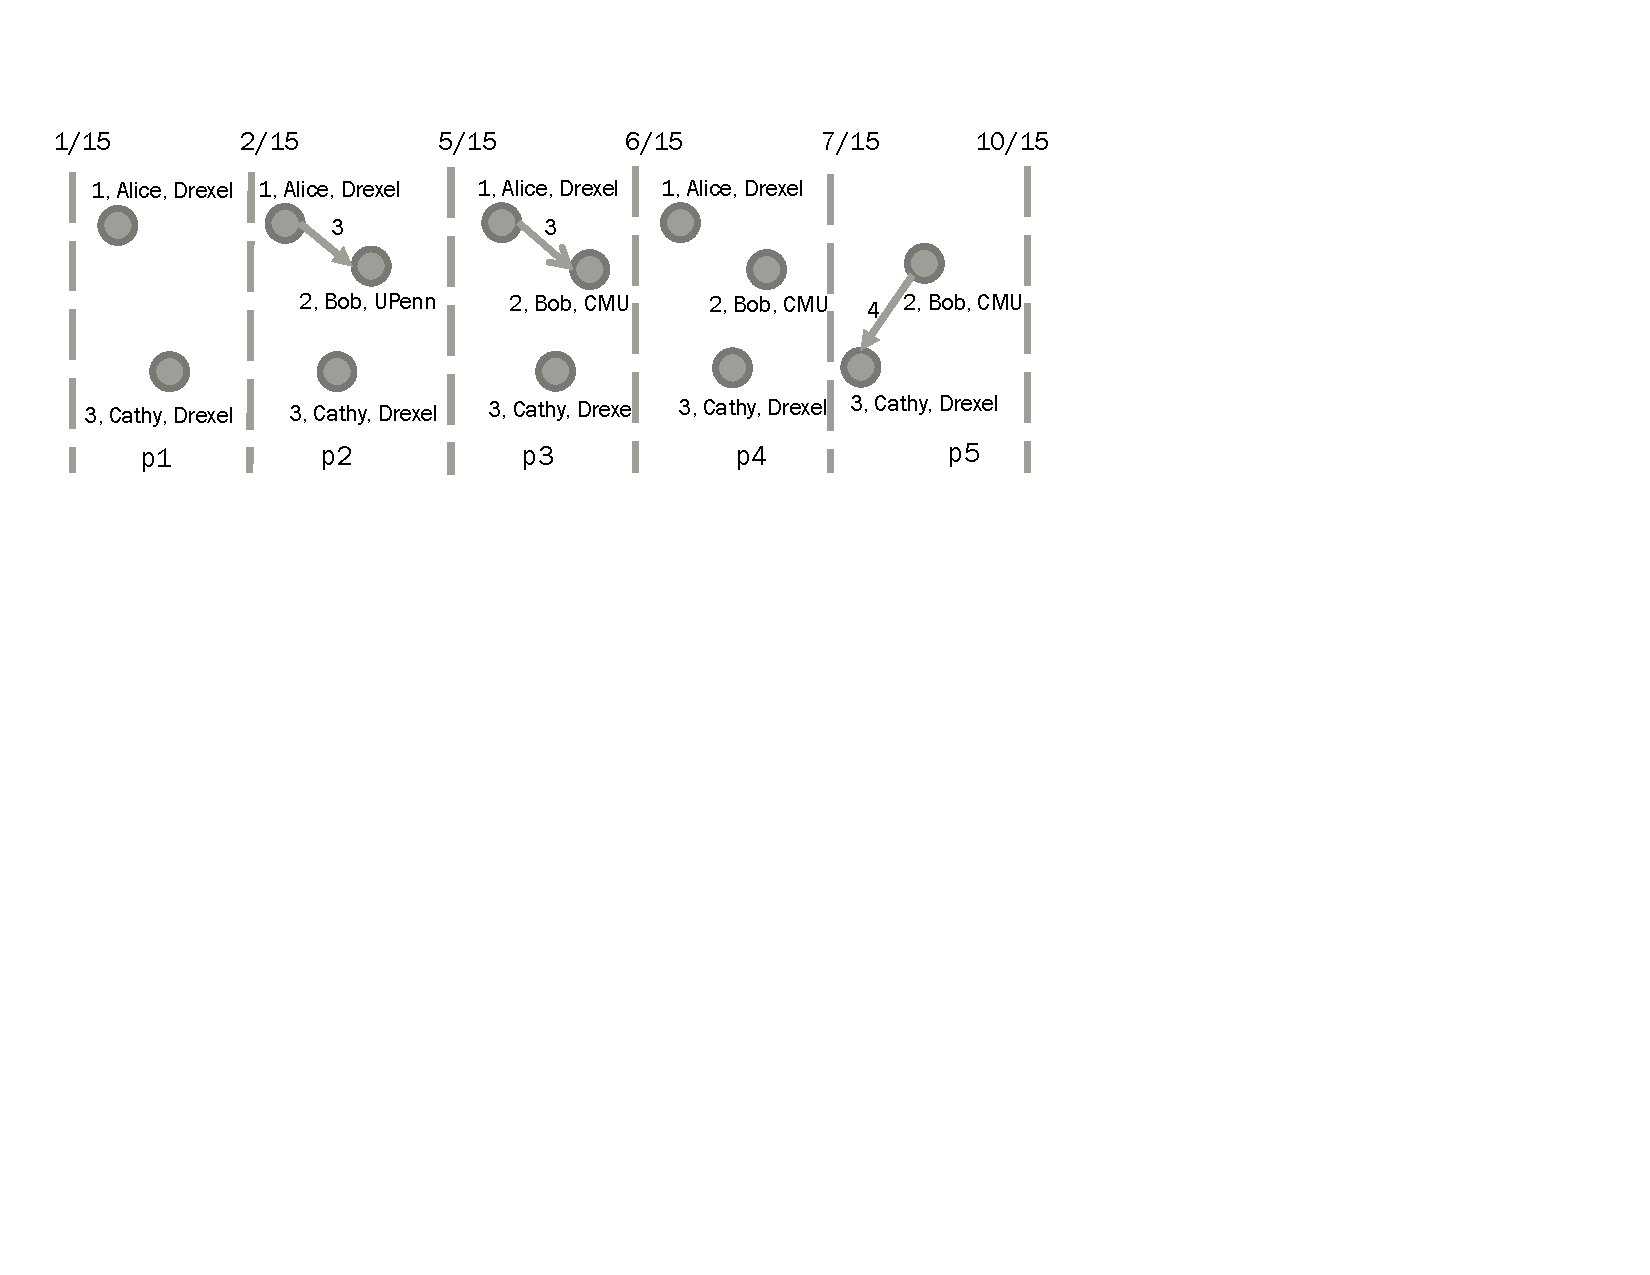
\includegraphics[width=3.5in]{figs/T1_graphs.pdf}
\caption{Representative graphs of \tg \insql{T1}.}
\label{fig:tg_rg}
\end{figure}

\begin{figure}
\centering
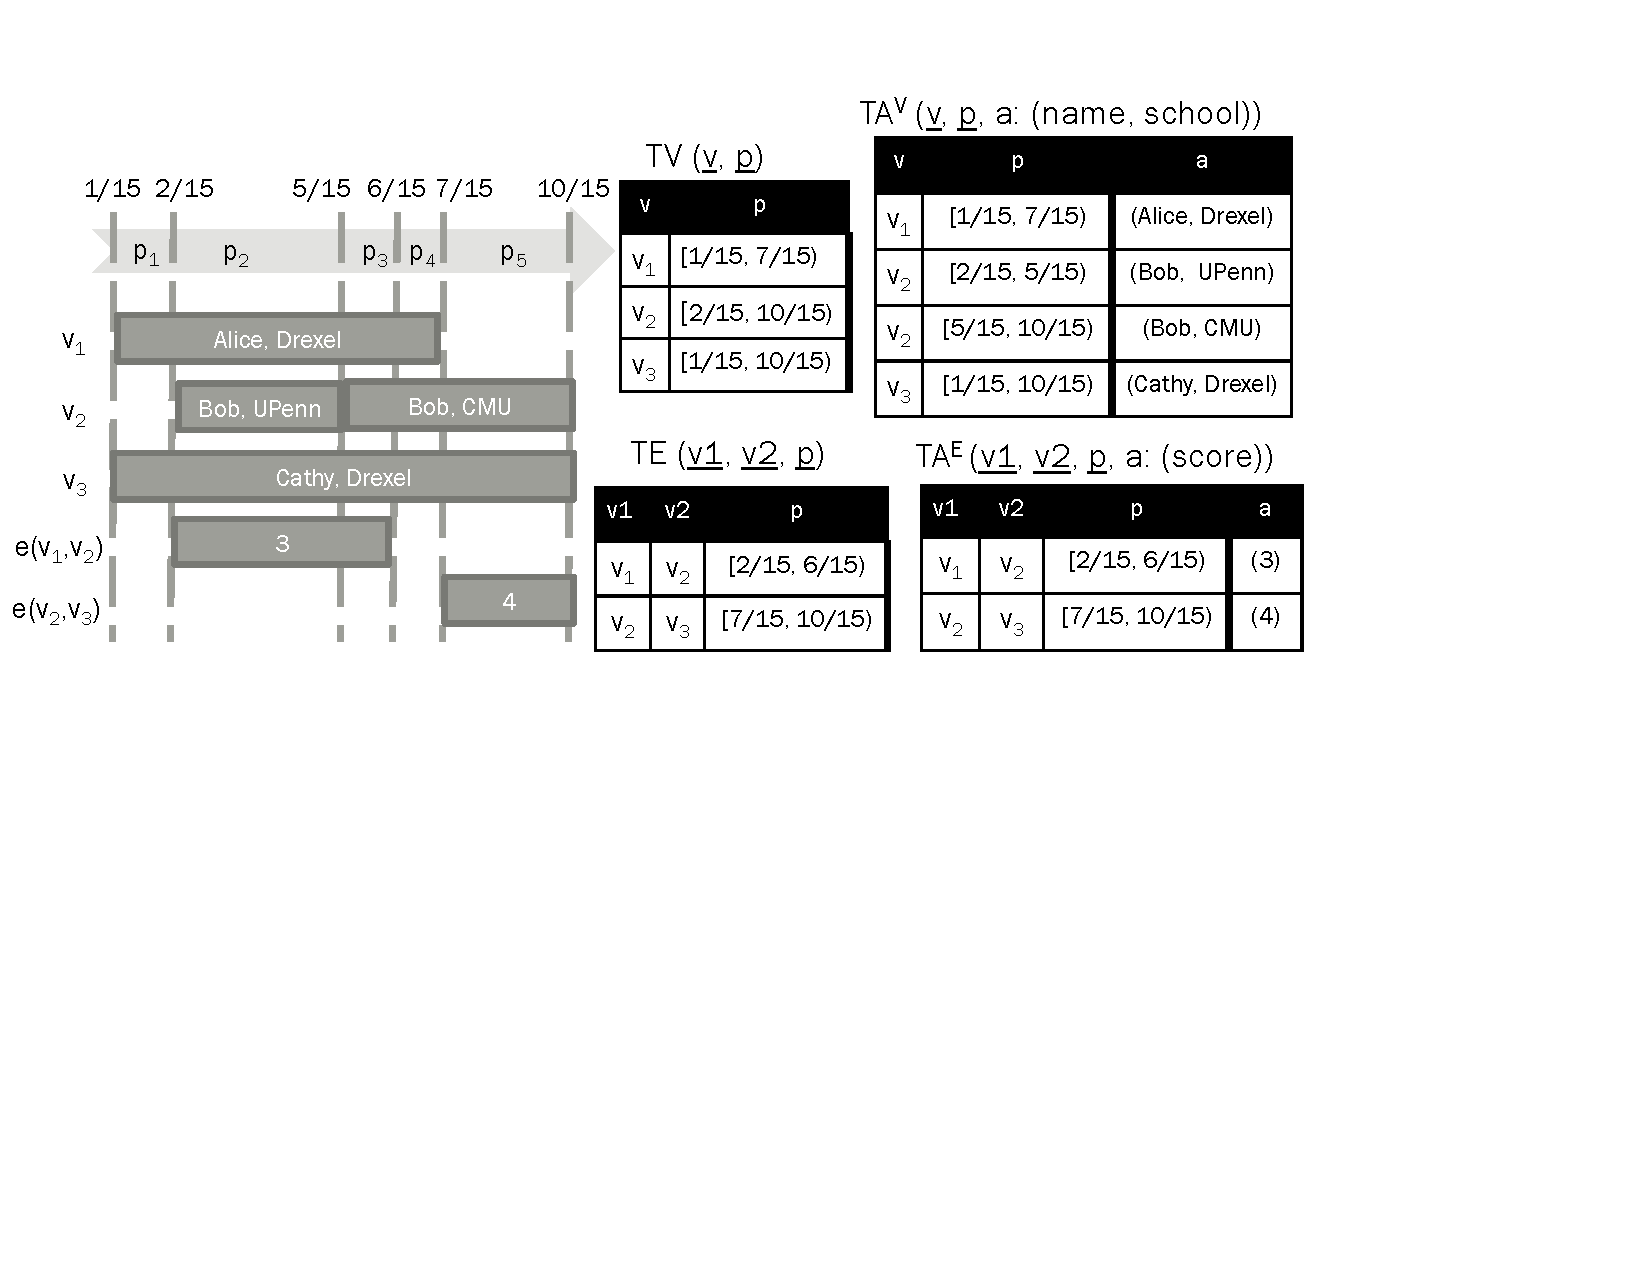
\includegraphics[width=3.5in]{figs/T1_rel_tab.pdf}
\caption{\tg \insql{T1}.}
\label{fig:tg_ve}
\end{figure}

\eat{It will be useful to quantify relationships between time periods $p$
and $q$ using the following Allen's relations~\cite{allen83}.}

\eat{\begin{itemize}
\item $p equal q$, defined as $p.start = q.start \wedge p.end = q.end$
\item $p overlaps q$, defined as $p.end > q.start$
\item $p meets q$, defined as $p.end = q.start$
\item $p during q$, defines as $p.start > q.start \wedge p.end < q.end$ 
\item $p starts q$, defined as $p.start = q.start \wedge p.end < q.end$
\item $p finishes q$, defined as $p.start > q.start \wedge p.end = q.end$
\end{itemize}}

We are now ready to present the basic building block of our model,
called a \tg.  

\begin{definition}[TGraph]
A \tg $T(g:graph, p:period) = \{ (g,p) \}$ is a coalesced valid-time
period-based relation in which a tuple associates a state of the graph
$g$ with a time period $p$ during which the graph is in that state.
We refer to each $g$ that appears in some tuple $(g,p)$ of $T$ as a
representative graph of $T$ during period $p$.
\label{def:tg_abstract}
\end{definition}

An example of a \tg is given in Figure~\ref{fig:tg_rg}, where 5
representative graphs (states) of \insql{T1} are associated with 5
consecutive time periods $[p_1=t_0,t_1), \ldots, p_5=[t_4,t_5)$.  As
    is typically the case in interval-based models, we assume that
    each representative graph exists continuously, and remains
    unchanged, during the associated period.  Note that it is not
    required that time periods in $T$ be consecutive and with no gaps.

To make the model of Definition~\ref{def:tg_abstract} more concrete,
and to help specify semantics of \tg operations, we will use
valid-time temporal SQL relations~\cite{DBLP:conf/vldb/BohlenSS96} to
represent evolution of graph topology, of its vertex and edge schemas,
and of values of its vertex and edge attributes.  This representation,
which we term the {\em \ve \tg}, is still a logical representation,
whith multiple possible physical representations.

An example of a \ve representation of a \tg is given in
Figure~\ref{fig:tg_ve}.  In its basic form, a \tg is represented by a
pair of temporal SQL relations $V$ and $E$ that capture evolution of
graph topology.  A \tg may optionally represent evolution of vertex
and edge attributes with relations $A^{V}_1, \ldots, A^{V}_n$ and
$A^{E}_1, \ldots, A^{E}_m$.

\eat{ Following notation in~\ref{DBLP:conf/vldb/BohlenSS96}, we will
  make use of $value\_equivalent(x,y) = (x[A] = y[A])$ --- a boolean
  predicate that evaluates to true of $x$ and $y$ agree on values of
  their explicit (non-temporal) attributes.}

\begin{definition}[Vertex-Edge TGraph]
A vertex-edge representation of \tg is a pair $T=(V; E)$, where $V$ is
a finite set of vertices with schema $V(\underline{v}, \underline{p})$
and $E$ is a finite set of edges connecting pairs of vertices from
$V$, with schema $E(\underline{v_1}, \underline{v_2}, \underline{p})$.
Attribute $p$ represents time period (as per Def.~\ref{def:period}).
Both $V$ and $E$ are coalesced:

\begin{multline}
\forall V(v, p)~~\nexists V(v, p')~~| \\
                       \pred{p}{meets}{p'}~\lor~\pred{p}{contains}{p'}~\lor~\pred{p}{overlaps}{p'}
\label{def:tg:c2}
\end{multline}
\vspace{-0.5cm}
\begin{multline}
\forall E(v_1, v_2, p)~~\nexists E(v_1,v_2, p')~~| \\
                       \pred{p}{meets}{p'}~\lor~\pred{p}{contains}{p'}~\lor~\pred{p}{overlaps}{p'}
\label{def:tg:c3}
\end{multline}

An edge connects a pair of vertices that exist at the time when the edge exists:
\begin{multline}
\forall E(v_1, v_2, p)~~\exists V(v_1, p_1), V(v_2, p_2)~~| \\
                       \pred{p_1}{contains}{p}~\wedge~\pred{p_2}{contains}{p}
\label{def:tg:c1}
\end{multline}
\vspace{-0.5cm}

\insql{T} optionally includes a collection of vertex attribute
relations $A^{V}_i(\underline{v},\underline{p},a)$ and edge attribute
relations
$A^{E}_j(\underline{v_1},\underline{v_2},\underline{p},a)$. Each
$A^{V}_i$ is coalesced, and assigns attribute values to existing
vertices.
\begin{multline}
\forall A^{V}_i(v, p, a)~~\nexists A^{V}_i(v, p', a)~~| \\
                       \pred{p}{meets}{p'}~\lor~\pred{p}{contains}{p'}~\lor~\pred{p}{overlaps}{p'}
\label{def:tg:c4}
\end{multline}
\begin{multline}
\forall A^{V}_i(v, p, a)~~\exists V(v,p')~~|~~\pred{p'}{contains}{p}
\label{def:tg:c5}
\end{multline}
Each $A^{E}_j$ is coalesced, and associates attribute values with
existing edges.
\begin{multline}
\forall A^{E}_i(v_1, v_2, p, a)~~\nexists A^{E}_j(v_1, v_2, p', a)~~| \\
                       \pred{p}{meets}{p'}~\lor~\pred{p}{contains}{p'}~\lor~\pred{p}{overlaps}{p'}
\label{def:tg:c6}
\end{multline}
\begin{multline}
\forall A^{E}_j(v_1, v_2, p, a)~~\exists E(v_1,v_2,p')~~|~~\pred{p'}{contains}{p}
\label{def:tg:c7}
\end{multline}

\label{def:tg}
\end{definition}

Graphs may be directed or undirected.  For undirected graphs we choose
a canonical representation of an edge, with $v_1 \leq v_2$ (self-loops
are allowed).

Conditions~\ref{def:tg:c2} and~\ref{def:tg:c3} in
Definition~\ref{def:tg} state that the \tg is
coalesced~\cite{DBLP:conf/vldb/BohlenSS96}, i.e., that each entity
(vertex or edge) is represented exactly once for each time period of
maximal length when it is present.  Conditions~\ref{def:tg:c4}
and~\ref{def:tg:c6} state that all attribute relations are coalesced,
i.e., that an attribute is represented exactly once for each time
period of maximal length in which its value did not change.

Consider the contents of $V$ and $E$ relations of \insql{T1} in
Figure~\ref{fig:tg_ve}, and note that there is a single tuple
corresponding to vertex $v_2$ in $V$, but two tuples corresponding to
$v_2$ in $A^{V}$, because the value of $a.school$ changed at time
$t_3$.

Definitions~\ref{def:tg_abstract} (\rgs) and~\ref{def:tg} (\ve) give
two alternative views of graph evolution.  In
Definitions~\ref{def:tg_abstract} the graph is represented in its
entirety, with a change of state occurring whenever there is a change
in graph topology or in its attribute schemas or values.  In other
words, time periods here are at their finest granularity.  In
contrast, Definition~\ref{def:tg} decouples evolution of graph
vertices, edes and attribute values, coalescing each relation
independently of the others.  This makes graph maintenance and
manipulation more manageable.  The \rgs represetation can be computed
from the \ve representation by (1) enumerating all time points during
which some change occured, i.e., that appear as either the start or
the end of some time period in $V$, $E$, or in any $A^{V}_i$ and
$A^{E}_j$; and (2) generating pairs of adjacent time points. See
Appendix for details.

{\bf Is temporal SQL enough?} The $V$ and $E$ relations of a \tg of
Definition~\ref{def:tg}, although only partially enforcing the
constraints, can be implemented as follows:

\eat{ Condition~\ref{def:tg:c1} in Definition~\ref{def:tg} states the
  natural integrity constraint that an edge linking two vertices can
  only exist during a time when both vertices exist. Here,
  $\pred{p}{contains}{q}$ is the Allen \predName{contains} relation
  with equality~\cite{allen83}, defined as $p.start \leq q.start
  \wedge p.end \geq q.end$.  Consider the vertex-edge representation
  of \tg \insql{T1} in Figure~\ref{fig:tg_ve}, where edge $e(v_1,v_2)$
  exists during the entire period when both $v_1$ and $v_2$ exist,
  while edge $e(v_2,v_3)$ exists only for a portion of the period when
  both $v_2$ and $v_3$ exist.}

\begin{small}
\begin{verbatim}
CREATE TABLE V (
  v LONG,
  pstart DATE,
  pend DATE,
  PERIOD for p (pstart, pend),
  PRIMARY KEY (v, p WITHOUT OVERLAPS) )

CREATE TABLE E (
  v1 LONG,
  v2 LONG,
  pstart DATE,
  pend DATE,
  PERIOD for p (pstart, pend),
  PRIMARY KEY (v1, v2, p WITHOUT OVERLAPS),
  FOREIGN KEY (v1, PERIOD p) REFERENCES V(v, PERIOD p),
  FOREIGN KEY (v2, PERIOD p) REFERENCES V(v, PERIOD p) )
\end{verbatim}
\end{small}

Unfortunately, this implementation does not guarantee that $V$ and $E$
are properly coalesced.  It does ensure that time periods
corresponding to a vertex (resp. edge) do not overlap, and that one
does not contain the other, but it does not prevent the existence of
two adjacent time periods for a vertex or edge, i.e., periods $p$ and
$q$ for which $\pred{p}{meets}{q}$.  That is, there may well be two
tuples in $V$ for $v_1$ in Figure~\ref{fig:tg+ve}, one associated with
$[t_0,t_1)$ and the other with $[t_1,t_4)$.

Another limitation of temporal SQL is that it does not provide a
convenient and efficient implementation of the coalesce operator
(see~\cite{DBLP:reference/db/Bohlen09} for possible implementations).
Coalescing requires that the system automatically merge adjacent and
overlapping time periods.  This operation, which is similar to
duplicate elimination in conventional databases, has been extensively
studied in the
literature~\cite{DBLP:conf/vldb/BohlenSS96,DBLP:journals/sigmod/Zimanyi06},
but is not supported by the SQL:2011 standard.  Note that, while it is
an important property of our logical model that time periods be
coalesced, eagerly coalescing is both expensive and, in some cases,
unnecessary.  We will discuss this when presenting \tg algebra
(Section~\ref{sec:algebra}) and its implementation in scope of Apache
Spark / GraphX (Section~\ref{sec:system}).

{\bf More about vertex and edge attributes.} While our \ve
represenation is based on temporal SQL, we remark here that non-key
attributes of vertices and edges are not restricted to be of atomic
types, and may, e.g., be lists, maps or tuples. This is illustrated by
relation $A^V$ in Figure~\ref{fig:tg_ve}.

Definition~\ref{def:tg} gives a columnar representation of vertex and
edge attributes.  Such a representation naturally supports {\em schema
  evolution} and can lead to more efficient physical representations,
especially when values of different attributes change at different
rates.  That said, our support of non-atomic types allows to combine
multiple, or even all, vertex (resp. edge) attributes in a single
attribute relation, as is the case in $A^V$ Figure~\ref{fig:tg_ve}.

Our choice to use attribute relations is in contrast to representing
vertex and edge attributes as part of $V$ and $E$.  The main reason
for this is to streamline the enforcement of referential integrity
constraints of Definition~\ref{def:tg}.  Consider again the example in
Figure ~\ref{fig:tg_ve}.  If vertex attributes were stored as part of
$V$, then there would be two tuples for $v_2$ in this relation, one
for each $[t_1, t_2)$ and $[t_2, t_5)$.  This would in turn require
    that $e(v_1, v_2)$ be mapped to two tuples in $V$ as part of
    referential integrity checking on $v_2$.  Matching a tuple with a
    set of tuples in the referenced table, while supported by the
    SQL:2011 standard, is both inelegant and potentially inefficient,
    and we avoid it in our representation.  We will discuss how
    integrity of the model is enforced, and how this is implemented,
    in Sections~\ref{sec:algebra} and~\ref{sec:system}.

\eat{ Non-key attributes of $V$ and $E$ are not restricted to be of
  atomic types, but may, e.g., be maps or tuples.  Because of this,
  \ql supports {\em schema evolution} in a \tg in much the same way as
  is done in popular (non-temporal) graph databases like Neo4j.  At an
  extreme, the vertex (resp. edge) relation will have a single
  unstructured non-key attribute, which would store all attribute
  information.  This representation has the usual advantages and
  disadvantages --- flexibility of a schema-less representation at the
  expense of missed performance optimization opportunities afforded by
  a structured representation.}

\eat{
To conclude this section, let us revisit \tg \insql{T1} in
Figure~\ref{fig:tg_ve}.  Figure~\ref{fig:tg_rg} represents \insql{T1} as a
continuous sequence of graph states, each corresponding to a time
period during which no change occurred to the graph, in terms of
either topology or attribute values.}

\eat{\begin{definition}[\rgs]
A {\em representative graphs} view of a \tg is a sequence of
(non-temporal) graphs associated with a sequence of consecutive
non-overlapping time periods.
\label{def:rgs} 
\end{definition}}

\eat{This view, to which we refer as \rgs of \insql{T1}, is computed from
properly coalesced $V$, $E$, $A^{V}$, and $A^{E}$ by (1) enumerating
all time points during which some change occured, i.e., that appear as
either the start or the end of some time period, and (2) generating
pairs of adjacent time points. See Appendix for details.  \rgs is an
important abstraction that will be useful to us in the next section,
where we present \tg algebra.
}
